\documentclass[12pt,compress]{beamer}
\usepackage{amsmath}
\usepackage{cmbright}
\usepackage{url}
\usepackage{ucs}
\usepackage[utf8x]{inputenc}
\usepackage[ngerman]{babel}
\usepackage{bbm}
\usepackage{ulem}
\usepackage{multicol}
\usepackage{comment}
\usepackage{setspace}
\usepackage{color}
\usepackage{media9}
\usepackage{hyperref}
\usepackage{bookman}

\usetheme{Boadilla}
\setbeamertemplate{footline}%{infolines theme}

\usecolortheme{lily}
\usefonttheme{serif}
\useinnertheme{circles}
\setbeamercovered{transparent}
\beamertemplatenavigationsymbolsempty

\definecolor{darkgreen}{rgb}{0,0.5,0}

\hypersetup{
    bookmarks=true,
    unicode=true,
    pdftoolbar=true,
    pdfmenubar=true,
    pdffitwindow=false,
    pdfstartview={FitH},
    pdftitle={Stabilität invertierter Pendel},
    pdfauthor={Michael Hartmann},
    pdfsubject={Vortrag über Stabilität invertierter Pendel},
    pdfcreator={vim},
    pdfproducer={pdflatex},
    pdfkeywords={Mathieu} {Stabilität} {invertierte Pendel},
    pdfnewwindow=true,
    colorlinks=true,
    linkcolor=black,
    citecolor=green,
    filecolor=magenta,
    urlcolor=darkgreen
}



\title{Stabilität invertierter Pendel}
\institute{Kaffeeseminar}
\author{Michael Hartmann}
\date{4. November 2016}


\titlegraphic{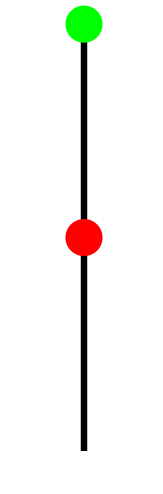
\includegraphics[scale=0.3]{images/title.png}}


\begin{document}

\begin{frame}
    \titlepage
\end{frame}


\frame{
    \frametitle{Überblick}
    \tableofcontents 
}

\section{Was ist ein Doppelpendel?}

\frame {
    \frametitle{Was ist ein Doppelpendel?}

    \begin{minipage}[b]{0.3\textwidth} 
    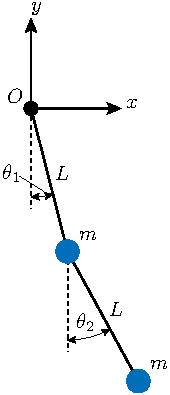
\includegraphics[scale=1.1]{images/sketch.pdf}
    \end{minipage}
    \hfill
    \begin{minipage}[b]{0.6\textwidth}
	Koordinaten
    \begin{align}
    \nonumber
    x_1 &= L \sin\theta_1 \\
    \nonumber
    y_1 &= -L \cos\theta_1 \\
    \nonumber
    x_2 &= L \sin\theta_1 + L \sin\theta_2 \\
    \nonumber
    y_2 &= -L \cos\theta_1 - L \cos\theta_2
    \end{align}

    \vfill

    Lagrange-Funktion
    \begin{align}
    \nonumber
    \mathcal{L} &= T-V \\
    \nonumber
    T &= \frac{1}{2} m v^2 \\
    \nonumber
    V &= mgL \left( 3-2\cos\theta_1-\cos\theta_2\right)
    \end{align}
    \end{minipage}
}

\frame {
    \frametitle{Normalkoordinaten}

    \only<1>
    {
    Kinetische Energie
    \begin{equation}
    \nonumber
    T = \frac{1}{2} m \left( \dot x_1^2 + \dot y_1^2 + \dot x_2^2 + \dot y_2^2\right) 
    \approx \frac{1}{2} mL^2 \left( 2\dot\theta_1^2  + \dot\theta_2^2 + \dot\theta_1\dot\theta_2\right)
    \end{equation}

    \vfill

    Potentielle Energie
    \begin{equation}
    \nonumber
    V = mgL\left(3-2\cos\theta_1-\cos\theta_2\right) \approx mgL\left(\theta_1^2 + \frac{\theta_2^2}{2} \right)
    \end{equation}

    \vfill
    }

    Lagrange-Funktion
    \begin{equation}
    \nonumber
    \mathcal{L} = T-V \approx \frac{1}{2} mL^2 \left( 2\dot\theta_1^2  + \dot\theta_2^2 + \dot\theta_1\dot\theta_2\right) - mgL\left(\theta_1^2 + \frac{\theta_2^2}{2} \right)
    \end{equation}

    \only<2>
    {
    \vfill

    Euler-Lagrange-Gleichungen
    \begin{equation}
    \nonumber
    \frac{\mathrm{d}}{\mathrm{d}t} \frac{\partial\mathcal{L}}{\partial\dot\theta_j} - \frac{\partial\mathcal{L}}{\partial\theta_j} = 0
    \end{equation}

    Linearisierte Bewegungsgleichungen
    \begin{equation}
    \nonumber
    \frac{L}{2g}
    \begin{pmatrix}
    2 & 1 \\
    2 & 2
    \end{pmatrix}
    \begin{pmatrix}
    \ddot \theta_1 \\ \ddot \theta_2
    \end{pmatrix}
    =
    -\begin{pmatrix}
    \theta_1 \\ \theta_2
    \end{pmatrix}
    \end{equation}
    }

    \only<3>
    {
    \vfill
    Eigenfrequenzen
    \begin{itemize}
    \item $\omega_1 = \sqrt\frac{2g}{L\left( 2+\sqrt{2} \right)} $
    \item $\omega_2 = \sqrt\frac{2g}{L\left( 2-\sqrt{2} \right)} $
    \end{itemize}

    \vfill

    In Normalkoordinaten
    \begin{equation}
    \begin{pmatrix}
    \omega_1^{-2} & 0 \\
    0 & \omega_2^{-2}
    \end{pmatrix}
    \begin{pmatrix}
    \ddot X_1 \\ \ddot X_2
    \end{pmatrix} =
    -\begin{pmatrix}
    X_1 \\ X_2
    \end{pmatrix}
    \end{equation}
    }
}

\frame {
    \frametitle{Indischer Seiltrick}

    \begin{center}
    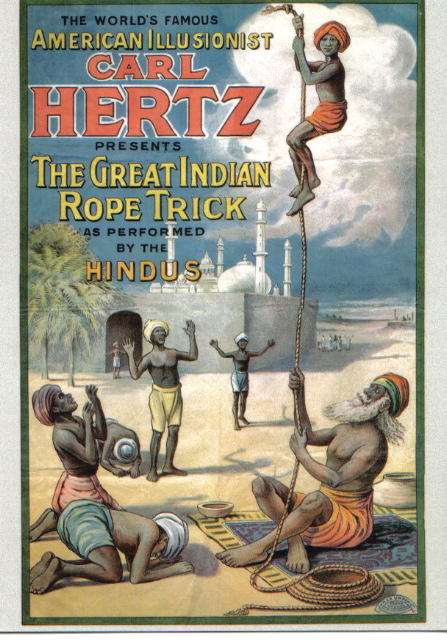
\includegraphics[scale=0.7]{images/Indian-Rope-Trick.jpg}
    \end{center}
}

\end{document}
